\section{DSL-Router und Computer vorbereiten}
Um als vollwertiger Teilnehmer an einem anonymen Peer-2-Peer Netz teilzunehmen, muss der eigene Rechner vom Internet aus erreichbar sein. Nur dann k�nnen andere Teilnehmer des Netzes den eigenen Knoten kontaktieren. Als typischer Heimnutzer mit DSL-Anschluss sind einige Anpassungen n�tig, damit der eigene Rechner aus dem Internet erreichbar ist.

\begin{enumerate}
 \item Der DSL-Router muss den ankommenden Datenverkehr der anderen Peer-2-Peer Teil�nehmer an den eigenen Rechner weiterleiten. Einige Programme k�nnen den Router mit UPnP konfigurieren. Aufgrund der Sicherheitsprobleme bei UPnP \footnote{ \href{http://heise.de/-1793625}{http://heise.de/-1793625}} sollte man dieses Feature auf dem Router deaktivieren und Weiterleitung per Hand konfigurieren.\\

Der Screenshot \ref{portforward} zeit die Konfiguration f�r einen Linksys Router. F�r I2P wurde im Beispiel der Port 8888 gew�hlt, f�r GnuNet muss man die Ports 1080 und 2086 weiterleiten. 
\begin{figure}[htb]
\begin{center}
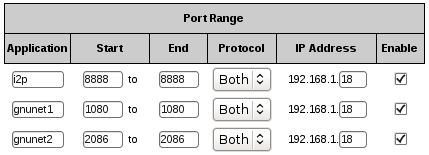
\includegraphics[scale=0.75]{../screenshots/router-portforward.png}
\caption{Portforwarding auf dem Router}
\label{portforward}
\end{center}
\end{figure}

 \item Die Konfiguration der Weiterleitung auf dem DSL-Router ist einfacher, wenn der eigene Rechner innerhalb des privaten lokalen Netzwerkes eine feste IP-Adresse hat. Daf�r �ndert man die Konfiguration der Netzwerkschnittstelle von \textit{DHCP} auf \textit{feste IP-Adresse}. 

 \item Au�erdem muss die Firewall auf dem lokalen Rechner den ankommenden Datenverkehr der anderen Peer-2-Peer Teilnehmer auf den Ports durchlasssen, f�r die eine Weiterleitung im Router konfiguriert wurde.

 \item F�r GnuNet und Freenet braucht eine DNS-Namen, um bei wechselnden IP-Adressen unter einer festen Adresse erreichbar zu sein. Mit einem DynDNS-Service kann man dieses Problem l�sen. Es gibt meherere freie DynDNS Dienste \footnote{ \href{http://dnslookup.me/dynamic-dns/}{http://dnslookup.me/dynamic-dns}} f�r diesen Zweck. (F�r I2P nicht n�tig!)
\end{enumerate}
